%29/10 - Paco Jurado
\chapter{Extracción de información}
\section{El problema de la extracción de información}
\subsection{Extracción}
Tenemos muchos documentos y la intención es automatizar la construcción de una base de datos de conocimiento estructurado. Se puede trabajar con documentos sencillos o múltiples. 

Las entidades son únicas, como son personas, lugares, organizaciones y fechas. Las relaciones incluyen un predicado y dos argumentos. Los eventos incluyen distintos tipos de argumentos, como por ejemplo un libro tiene un título, autor y fecha de salida. 

La extracción de información no es igual a la recuperación de información. La extracción obtiene información relevante de documentos basado en un análisis lingüístico del texto. Por el contrario, la recuperación de información obtiene los documentos relevantes de una colección, utilizando generalmente modelos de bag of words.

Tras la extracción de la información, se debe guardar en alguna base de datos que permita posteriormente realizar búsquedas. Primero se suelen reconocer las entidades para posteriormente buscar la relación entre las distintas entidades. 

\subsection{Bases de conocimientos}
La DBpedia es la ontología de la Wikipedia. Incluye la información de Wikipedia estructurada en forma de pares de propiedades y valores. Básicamente incluye los infoboxes que aparecen en el recuadro de cualquier página de Wikipedia, tablas, listas, etc. No está en una base de datos per se, si no que está en formados basados en XML como RDF u OWL. Los datos RDF consisten de tripletes sujeto predicado objeto. Esto es lo que tiene la DBpedia pero a gran escala. El lenguaje de consulta es SparkQL.

WordNet también es una base de conocimiento léxica. Otros ejemplos son Yago, Freebase o Linked Open Data.

\section{Tarea de extracción de información}
\subsection{Reconocimiento de entidades}
El reconocimiento de entidades nombradas es un problema recurrente. La idea es poder identificar dentro de un texto las personas, lugares, fechas, organizaciones etc que aparecen en el mismo. En la mayoría de los parsers son personas, organizaciones, lugares, geopolíticos y misceláneos. Para abordar el problema de reconocer y asignar la etiqueta no se puede enfocar solo en las mayúsculas, aunque sí puede ayudar como primera aproximación. Además, hay que tener en cuenta la delimitación por conjunciones, como por ejemplo en "Hospital Ramón y Cajal". Un tipo común de ambiguación es en personas vs organizaciones vs entidades geopolíticas y depende del contexto.

Para afinar la extracción se busca capitalización, presencia de palabras clave alrededor (como "señor" antes del nombre de una persona), etc. En algunas ocasiones se utilizan gazetteers, que son listas de nombres de personas, lugares, códigos postales, etc para poder comparar con lo que aparezca en un documento. Su ventaja es que son rápidos y fáciles de implementar en todos los idiomas, pero no es posible enumerar todos los nombres ni variantes, hay posibles ambigüedades de nombres que aparezcan en más de un listado, etc. 

Algunas aproximaciones se basan en machine learning para entrenar un algoritmo que ayude a segmentar la información (tarea de etiquetado de secuencias). Entre ellos se encuentran HMM, CRF y RNN. El procedimiento estándar es IO (in out), BIO (begin in out) y BIOES (begin in out end single). Esto identifica en el texto cuándo está dentro de algo etiquetado como persona, fuera, dentro de algo etiquetado como organización, etc. 

\begin{figure}[h]
\centering
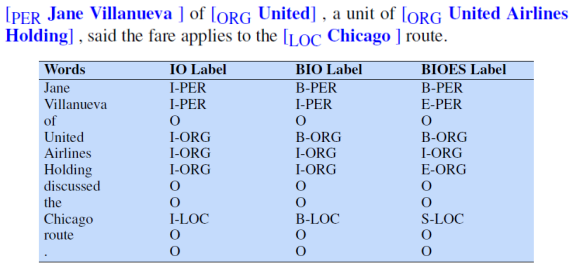
\includegraphics[width = 0.8\textwidth]{figs/bioes.png}
\end{figure}

Una vez que está todo etiquetado se utilizan los algoritmos analizadores para etiquetar texto nuevo y construir la base de conocimiento. La wikificación es la identificación de personas y fechas y buscar en la wikipedia si existe para poner el vínculo. De esta forma se añade información sobre el texto. En eso consiste el texto de lincado de entidades (entity linking). En la wikificación, se crea una estructura similar a un diccionario en el cual se utilizan los nombres de las páginas como nombre de las entidades. Además, incluye las páginas de redireccionado con nombre alternativos y páginas de desambigüación para entidades que comparten el nombre. En el propio texto hay muchos enlaces adicionales para poblar la base de conocimiento. Las palabras en negrita dan más información sobre el propio término. Con esto se pueden unir las distintas entidades, ya que el texto está semiestructurado. Hay algunos algoritmos de lincado automático usando redes neuronales.

\subsection{Reconocimiento de expresiones temporales}
Generalmente hay tres tipos de expresiones temporales: fechas y horas absolutas que se pueden mapear directamente al calendario, tiempos relativos vinculados con un momento anterior o posterior (la semana pasada, el próximo martes, etc.) para los que se debe conocer el momento actual para hacer los cálculos, y duraciones (durante 15 días, etc.). Algunas palabras concretas pueden indicar expresiones temporales como los nombres de los meses o festividades (Navidad, Ramadan), nombres de momentos del día (mañana, noche, amanecer). 

Las aproximaciones basadas en reglas utilizan cascadas para reconocer patrones con pequeñas reglas y expresiones regulares. Como alternativa se puede utilizar un parsing de texto BIO.

Esto nos lleva a tener que etiquetar de forma normalizada. Un estándar es TIMEX3 para etiquetar los momentos específicos en el tiempo. 

\subsection{Extracción de relaciones}
Tras reconocer las distintas entidades, el siguiente paso es encontrar las relaciones entre las mismas. Esto está muy vinculado con el RDF para establecer los enlaces entre la información. 

Las relaciones están estandarizadas. La ontología Automatic Content Extraction (ACE) cuenta con 17 relaciones semánticas.
Algunos datasets tienen relaciones etiquetadas manualmente para poder utilizar en el entrenamiento y test de algoritmos extractores. Un ejemplo es el TACRED dataset que tiene 106.264 ejemplos y reconoce 41 tipos de relaciones.  

Para hacer esto se puede utilizar aprendizaje automático o utilizar reglas mediante expresiones regulares o patrones. Con un corpus etiquetado, se recomienda utilizar un algoritmo de aprendizaje automático al ser más preciso, aunque depende del contexto se utiliza una aproximación u otra. 

\subsection{Detección de eventos}
Los eventos son las menciones a eventos en el texto. Siempre tiene un momento particular en el que se da el evento, pero normalmente se trata de verbos que introducen los eventos o informan de lo que ocurrió. 

Para clasificar los eventos se pueden etiquetar como acciones, estados, percepciones, etc. Al igual que antes se modelan mediante aprendizaje supervisado mediante el tagging BIO o clasificadores multiclase. Se puede registrar la clase, tiempo verbal y aspecto. 

\subsection{Completado de plantillas}
Una plantilla es una estructura de datos que describe eventos o situaciones recurrentes. Se compone de unos slots con forma de [nombre:valor]. El completado de la plantilla busca esos eventos y los rellena en los slots. 

Como entrada se necesitan los documentos etiquetados y se crean las plantillas de forma automática con machine learning. 